\subsection{Dependency Inversion Principle (DIP)}
DIP har følgende centrale punkter:\\

\textit{''High level modules should not depend on low level modules. Both should depend on abstractions.''}\\

\textit{''Abstractions should not depend upon details. Details should depend upon abstractions.''}\\

Det hedder dependency inversion fordi vi invertere afhængigheden for klasserne på figurene på side~\pageref{fig:dipright}. Sådan at afhængigheden fra figur~\ref{fig:dipwrong} bliver inverteret, som vist på figur~\ref{fig:dipright}.\\

\begin{figure}[H]
	\centering
	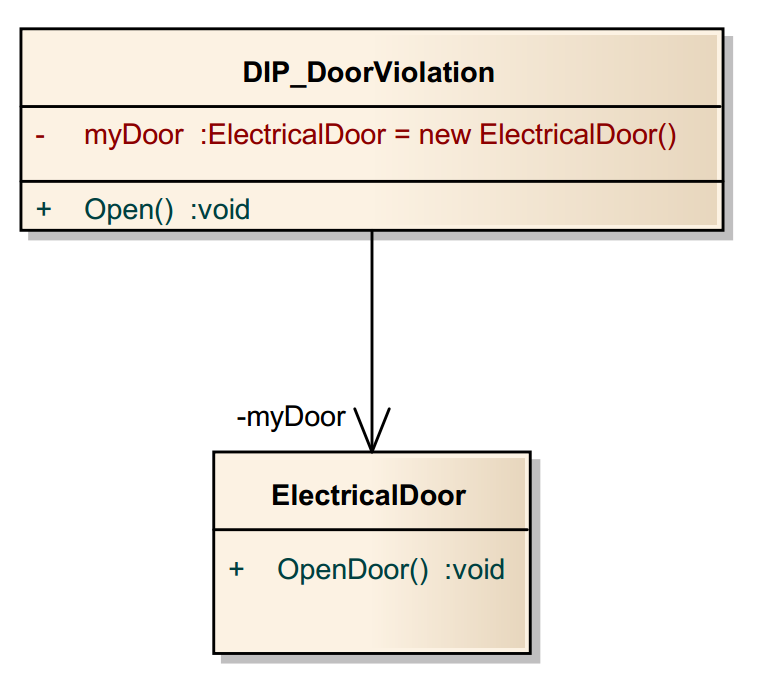
\includegraphics[width=0.6\linewidth]{figs/DIP/dipwrong}
	\caption[DIP eksempel 1]{Eksempel på klasser hvor DIP ikke er anvendt.}
	\label{fig:dipwrong}
\end{figure}

\begin{figure}[H]
	\centering
	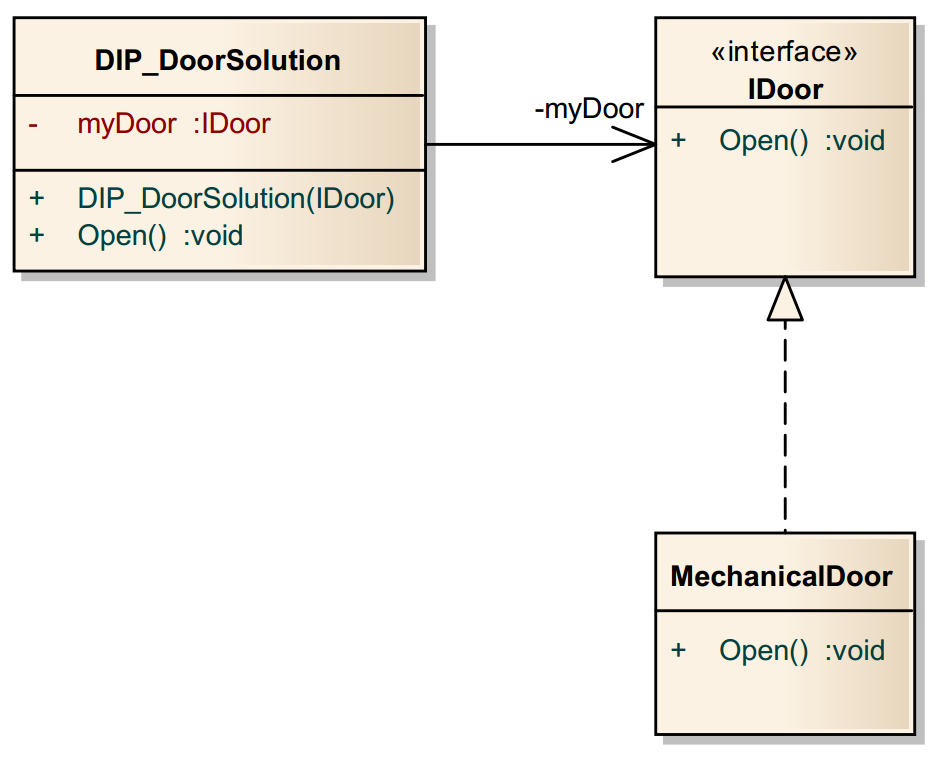
\includegraphics[width=0.6\linewidth]{figs/DIP/dipright}
	\caption[DIP eksempel 2]{Eksempel på hvor DIP er anvendt.}
	\label{fig:dipright}
\end{figure}

%Det der menes med abstraktioner her, er \textbf{interfaces}. Et eksempel på DIP er vores øvelse med Compressions Stocking, hvor vi fx havde nogen knapper (high-level) der kaldte noget low-level funktionalitetet, lader vi den afhænge af et interface.\\

Med andre ord så er det ikke vores high-level modul som opretter/indeholder low-level modulet. I stedet har den et interface, som dette low-level modul implementere.
På denne måde kan den underliggende funktionalitet let ændres/skiftes ud senere fordi high-level modulet ikke længere siger: “tænd for lampe”, men i stedet siger “lav lys” og så er det nu vores implementering af dette interface som afgør om det er en lampe der tændes eller et stearinlys.\\ 

Klassediagrammet kan ikke være på én side så derfor kan billedet for øvelsen kan ses på  \href{https://raw.githubusercontent.com/BjornNorgaard/I4SWD/bdd4a11a87f182d81b3ed81409a2052e45be82c3/Eksamen/Disposition/figs/compressionstockings_classdiagram.PNG}{dette billede} fra github repo'et.